\section{Computer Program Optimization} \label{app:opt}

When optimizing a program, there is an important cardinal rule to follow which at times
is easy to forget in the face of increasingly interesting and complex minor optimizations
designed to squeeze every bit of performance out of your computer. Unfortunately, due
to the complexity of modern computer hardware, it is
very difficult to predict if a given micro-optimization will actually be benificial or
not. For this reason, the most important rule when taking a working program and making it
fast is\footnote{besides \textit{don't break it}, of course. An incorrect program is worthless, no matter
how fast it is.} \textit{benchmark everything}.

The field of program optimization is huge. There is a small number of people who, for
a given platform, are really \textit{good} at optimization. There is an even smaller number
who are truly experts. I do not fit into either of these categories. For this reason, the program
that I have written here is \textit{decently} optimized. I believe that the maximum throughput
is not orders of magnitude better than what I have achieved, however, there is still a lot of work
that can be done (including a potentially significant optimization that I have neglected, and will talk
about later).

%TODO%%%%%%%%%%%%%%%%%%%%%%%%%%%%%%%%%%%%%%%%% ACTUALLY TALK ABOUT THAT ************************

\subsection{Lazy Programs Are Better}

Before taking up a sharp cutting tool and carving away a program to make it run faster, it helps to examine
what exactly is the program trying to accomplish and how. There are often multiple ways to solve a problem,
and some of them may be more efficient than others. In my case, I utilized two different methods of solving
a problem: Jacobi iteration and successive over-relaxation. One of them was significantly faster than the other
not because each iteration of the program was quicker but because it had to do less iterations. It was using a
smarter algorithm.

Computer scientists talk about algorithmic complexity using order notation. For example, given a random list
of numbers, if I want to test to see if a certain number if in the list, I need to look through the whole
list in order to check if it is there. This is an $O(n)$ operation, meaning that if the list is of size $n$, I
have to do $n$ operations to determine if the item is there or not. Data structures commonly have operations
associated with them, and those operations (such as \texttt{find}, \texttt{insert}, etc) have associated
time costs. Choosing the correct data structure for a problem is one of the first steps towards correctly
organizing a program for it to be efficient. If a program is constantly searching through a list to find
values when instead a simple hash table could be used, the program will run slowly. A program should not
do additional work when it does not need to. Only once the data structures have been properly designed
and the algorithms properly thought through should \textit{optimization} be done.

\subsection{Freebies}

There are some optimizations which can be used in high confidence and are also very easy to do.
The first, and most obvious, is to use a fast language. While writing in \texttt{C} may be a chore
compared to writing in python, the resulting code will be much faster. This is the reason behind the
organization of this program: the frontend (which has no performance requirements) is written in
python because parsing the configuration file is much easier. The backend needs to be fast, so it
is implemented in \texttt{C}.

A quick and rough experiement can easily convince you that this is true (remember how I said to
benchmark everything?). Credit to my friend Chris Milke for doing this test. Write the following
code in both python and in C: initialize a variable to zero. Then loop from zero to some large
number (we used 123,456,789), and add that iteration to the variable. After the loop, print the
variable. The resultant python program took 14.25 seconds to run on my computer, but the C code
completed \textit{instantaneously}. Why is python slower than C in general? Because python is
an interpreted language. The code that you write is read by another program and executed by
that program. In contrast, C code must be compiled into machine code. This is then run directly
on the processor, which cuts out the middle-man of the interpreter.

When using C, there are some more things that you can get for free: compiler optimizations. When
compiling a C program, the command looks something like this: \texttt{gcc -Wall -Wextra foo.c}\footnote{as an aside, you should \textbf{always} compile with -Wall and -Wextra, and eliminate all warnings from your program.
Warnings are warnings for a reason, and should rarely be ignored.}. This will
result in a compiled C program (a binary file, containing the machine code), but it will be
unoptimized. There are reasons why one may want an unoptimized binary (they are typically
easier to debug, for example), but generally when you compile your program for actual usage
you will want to optimize it. An aggressive optimization compilation command may look something
like: \texttt{gcc -Wall -Wextra -O3 -ffast-math -mavx}, as a start. The main flag here is \texttt{-O3}, which
enables almost every optimization that gcc can do.

Going back to the example from earlier, the optimized version of the C program completed instantly, but
the unoptimized version took 0.33 seconds. The unoptimized version is still 43 times faster than the
python code, but what was the optimizing compiler doing to make it so much faster with \texttt{-O3} on?
Part of optimizing is understanding why something is faster, so lets look at the assembly code. On \textsc{unix},
this can be done with the objdump command. Table \ref{table:assem-1} shows the annotated assembly from
the function \texttt{main}. If you don't know x86\_64 assembly language, you will at least notice that the
optimized version is much shorter. If you do know how to read the assembly, you'll notice that the unoptimized
version is doing almost literally what the C code says to do: set a variable to zero, and iterate from zero to
a big number, adding that iteration to the variable, and finally printing the variable. The optimized code just prints a large number -- which happens to be the result of the sum.

\begin{table}[h]
	\centering
\begin{tabular}{l | l}
	\hline
	\textbf{Unoptimized} & \textbf{Optimized}\\
	\hline
	\texttt{mov [rbp-0x10], 0x0}	&\texttt{movabs rsi,0x1b131147ee6b52} \\
	\texttt{jmp .loop\_end			}	&\texttt{mov edi,0x400594} \\
	\texttt{.loop\_top:                } &\texttt{xor eax,eax   } \\
	\texttt{mov rax, [rbp-0x10]				}	&\texttt{jmp 4003c0 <printf@plt>}\\
	\texttt{add [rbp-0x8], rax				}	&\texttt{	} \\
	\texttt{add [rbp-0x10], 0x1				}	&\texttt{ }\\	
	\texttt{.loop\_end:                       } &\texttt{} \\
	\texttt{cmp [rbp-0x10],0x75bcd14} &\texttt{} \\
	\texttt{jle loop\_top} &\texttt{} \\
	\texttt{mov rsi,[rbp-0x8]} &\texttt{} \\
	\texttt{mov edi, 0x4005b4} &\texttt{} \\
	\texttt{mov eax, 0} &\texttt{} \\
	\texttt{call 4003c0 <printf@plt>} &\texttt{} \\
\end{tabular}
	\caption{Unoptimzed and optimized assembly from the sum-a-lot-of-numbers example.}
	\label{table:assem-1}
\end{table}

This is just a simple example, but a good C compiler can drastically improve the performance of a
program. Here, it made a program that took a third of a second (which is already drastically faster than
the interpreted python version!) finish instantly.

\subsection{A Model of Processor Design}

When first learning to program in a language that does more accurately display what is going on
inside of a computer, it is helpful to have a mental model for what is going on during each
simple operation that a programmer might want to do. Since programs are sets of instructions
which define transformations on data, it is tempting to think about a model such as in figure~\ref{fig:1a},
where there is some nebulous device which follows your instructions and is connected to a large amount
of memory in which your variables and data structures live.

Unfortunately, while this is a convenient abstraction to think about programming up an application, it
is not actually what is going on\footnote{I do not claim that what I am about to describe is what is ``actually going on'' either,
but it is at least significantly less of a lie.}. A more realistic model is shown in figure~\ref{fig:1b}. There are
several key take aways from this. One of them is that RAM is \textit{really slow}. The second is that the processor
chip is aware that RAM is really slow and so it aggressively caches everything that it ever gets out of RAM. This diagram
shows the actual detailed level of caches that cores have on them, and that they have a shared cache, but most of that
complexity is not needed for a basic understanding. When one makes first steps towards optimizing a program, it is vital
to think in the more complex model, because a huge amount of time will be spent trying to optimize the program according
to how the processor actually works.

\begin{figure}[h]
\begin{subfigure}{0.4\textwidth}
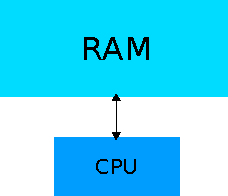
\includegraphics[width=\linewidth]{ram-cpu-simple.pdf}
\caption{Simplistic view of CPU and RAM.} \label{fig:1a}
\end{subfigure}
\hfill
\begin{subfigure}{0.4\textwidth}
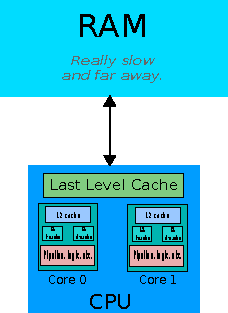
\includegraphics[width=\linewidth]{ram-cpu-complex.pdf}
\caption{More realistic view of CPU and RAM.} \label{fig:1b}
\end{subfigure}
\label{fig:cpu-and-ram}
\caption{View of programming that programmers like to have (a), versus the the more realistic
	and complicated view (b).}
\end{figure}

\subsubsection{Caching}

On modern processor chips, the vast majority of the silicon is used to implement a memory cache. This gives an indication
of how important it is. Think of the cache as a smaller, but much much faster memory that the processor accesses whenever
it would access RAM. If it finds the value in the cache, reading a value can take between 1 and 10's of nanoseconds. However,
if it does not find the value in the cache, it must then perform a read from memory, which can take hundreds of nanoseconds.
For scale, a single instruction very often takes less than a nanosecond to do. This means that if a program makes a lot of
memory accesses, the processor will spend a lot of time waiting and not much time calculating.

Earlier in this document, I described a phenomenon which describes how important caching is. Given a 2-D array, there are two
ways to iterate over the whole thing: line-by-line or column-by-column. On my computer, the line-by-line method was five times
faster than the alternative. This has to do with the cache, and specifically, \textit{cache lines}. When reading a value out
of memory for the first time, the processor actually reads many values, something like 64 bytes worth of data. This is fact
of the design of the hardware, and is partly because if you read a value $x$ from RAM, the processor expects you will want to
access memory that is nearby $x$ in the near future. Thus, if you iterate over an array line-by-line, when you access the
first element of a line you are actually reading in multiple elements of the array into the cache at once. When the processor
then tries to access the second element of the line, it finds that it is already in the cache, making that access much faster
than if it had not been in the cache. If you iterate over the array column-by-column, you read the first element of the line,
which loads several elements from that line into the cache, and then \textit{those values are ignored} and the first element
of the second line is read. This means that when reading the first element of the lines, each time the processor has to fetch
the value from RAM and does not get a chance to make use of the cache. By the time an entire column has been read, the cache
may be full, forcing the processor to remove old values from it. Then, when the program reads the second element of the first line,
that data no longer in the cache. This is extremely slow.

If possible, try to keep the amount of memory that the program accesses small. Try to organize the access patters such that it is
something that the processor is good at handling (like the iteration direction choice above). I have utilized these methods in my
solver program. An example for keeping memory footprint small was to reuse variables inside the grid that I knew were safe to reuse.
Additionally, I used \texttt{float}s instead of \texttt{double}s wherever possible, as this reduces memory usage as well.

\subsection{Structure of Arrays}

\subsection{Multithreading}

\subsection{Vectorization}
\subsubsection{Branch Reduction}



